\documentclass[thesismargins, thesislinespacing]{rnthesis}
\usepackage[slovak]{babel}
\usepackage[utf8]{inputenc}
\usepackage[]{graphicx}
\usepackage{nomencl}
\usepackage{lineno} 
\usepackage{caption}
\usepackage{subcaption}
\usepackage{braket}
\usepackage{multirow}

\title{Uhlové dvojhadrónové korelácie}
\author{Lucia Anna Husová}
\typprace{ŠVK}
\rok{2018}
\miesto{Košice}
\odbor{Fyzika}
\podakovanie{
Na tomto mieste sa chcem poďakovať vedúcemu mojej práce doc. RNDr. Marekovi Bombarovi, PhD. za odborné rady a   osobný prístup.  Taktiež sa chcem poďakovať priateľovi Martinovi a rodičom za osobnú podporu.  	
  
} 
\veduci{doc. RNDr. Marek Bombara, PhD.}
\pracovisko{Ústav fyzikálnych vied, Katedra jadrovej a subjadrovej fyziky}

\abstract{
	
	The low energy jets are hardly identified in heavy ions collisions due to high background and the possible shape deformation. Therefore the two-particle correlation method is used to study these low energy jets in heavy ions collisions.\\
	In this thesis, the results of two-particle correlation method applied on the proton-proton collisions data at 13~TeV collected by the ALICE experiment at the LHC are presented. The yields for near-side and away-side peak for unidentified trigger particles as a function of transversal momentum of trigger particles and multiplicity were measured. The structures of two-dimensional correlation function and the ratio of high-multiplicity and low-multiplicity yields were also studied. An increase of the near-side yield in high-multiplicity events with respect to low-multiplicity events is observed as well as a possible hint of away-side peak suppression.

}


\abstrakt{
	
	Nízkoenergetické jety vzniknuté v zrážkach ťažkých iónov sú ťažko identifikovateľné vzhľadom na vysoké pozadie a možnú deformáciu ich tvaru, preto sa na ich štúdium, najmä v zrážkach ťažkých iónov, využíva metóda dvojčasticových korelácií.\\
	V tejto práci sú prezentované výsledky metódy dvojčasticových korelácií aplikovanej na dáta z protónovo-protónových zrážok pri energii 13 TeV zozbieraných na experimente ALICE na urýchľovači LHC. Merané boli výťažky pre priľahlý aj protiľahlý pík pre neidentifikované trigrovacie častice v závislosti od priečnej hybnosti trigrovacích častíc a multiplicity zrážok. Skúmané boli aj štruktúry dvojrozmerných korelačných funkcií v závislosti od multiplicity a pomer výťažkov pre vysokomultiplicitné a nízkomultiplicitné zráž\-ky. Namerané bolo relatívne zvýšenie výťažkov vysokomultiplicitných zrážok ku nízkomultiplicitným pre priľahlý pík a náznak mierneho potlačenia pre protiľahlý pík.

\newpage
}

\makeglossary


\bibliographystyle{alpha}
%\linenumbers 
\begin{document}
\begin{center}
	{\Large Univerzita Pavla Jozefa Šafárika v Košiciach} \\
	%\end{center}
	%\begin{center}
	{\Large Prírodovedecká fakulta} 
\end{center}

\vspace*{2cm}

\begin{figure}[htbp!]
	\begin{center}
		
\includegraphics[width=3cm]{./Obrazky_praca/logo-pf-upjs-cb.jpg}
	\end{center}
\end{figure}

\vspace*{2cm}

\begin{center}
	%\vspace*{7cm}
	{\LARGE\bf Uhlové dvojhadrónové korelácie}
\end{center}

\begin{center}
	{\large ŠVK práca}
\end{center}

\vspace*{5cm}
\begin{flushleft}
{\bf Študijný odbor:}{ Jadrová a subjadrová fyzika} \\
{\bf Školiace pracovisko: }{Katedra jadrovej a subjadrovej fyziky}\\
{\bf Vedúci práce: }{doc. RNDr. Marek Bombara, PhD.}\\
\end{flushleft}
 
 \vspace*{2cm}
 \begin{flushleft}
{\large Košice 2018}
\hspace*{5cm}
{\large Bc. Lucia Anna Husová}
\end{flushleft}

\thispagestyle{empty}
\newpage

\maketitle
\newpage
\tableofcontents
\newpage

\chapter*{Úvod}
\addcontentsline{toc}{chapter}{Úvod}
Ani v súčasnej dobe nevieme nájsť odpovede na množstvo fundamentálnych otázok, preto si fyzika vysokých energií stále udržuje primát jednej z najaktívnejších oblastí fyziky. Na tento účel bol postavený najväčší urýchľovač častíc LHC (Large Hadron Collider) v laboratóriu CERN, ktorý nie je zameraný len na štúdium novej fyziky, ale aj na testovanie správnosti Štandardného modelu (ŠM) elementárnych častíc. Na LHC sa okrem protónovo-protónových zrážok skúmajú aj zrážky jadier olova, pri ktorých  sa vytvára kvarkovo-gluónová plazma (QGP), o ktorej sa predpokladá, že ňou bol tvorený Vesmír tesne po Veľkom tresku. 

Vlastnosti QGP sa vo väčšine prípadov skúmajú nepriamo prostredníctvom \-had\-ró\-nov, ktoré obsahujú kvarky a gluóny pochádzajúce z plazmy. Jedným z populárnych \-spô\-so\-bov sú tzv. "hard probes". Ide o rýchle partóny, ktoré interagujú s plazmou. Tie následne rozpoznávame v detektoroch ako spŕšky hadrónov (jety). Jety sa dajú skúmať \-pria\-mo alebo nepriamo, napr. metódou dvojčasticových korelácií. 

\chapter{Kvantová chromodynamika}

Po objave vnútornej štruktúry protónov v 60-tych rokoch minulého storočia v laboratóriu SLAC (Stanford Linear Accelerator Center) bolo potrebné vytvoriť teoretický model popisujúci správanie sa novoobjavených častíc - partónov, ktoré boli neskôr priradené k teoreticky predpovedaným kvarkom a gluónom. Na pochopenie interakcie medzi partónmi vznikla kvantová chromodynamika (QCD), ktorá bola sformulovaná na základe symetrií, podobne ako staršia kvantová elekrodynamika (QED). V QED je zdrojom vzájomného pôsobenia elektrický náboj. Jeho analógiou v QCD je farebný náboj ako zdroj silnej interakcie, ktorý môže nadobúdať šesť stavov (modrý, červený, zelený, antimodrý, antičervený, antizelený)\footnote{druhy farebného náboja nesúvisia s farbami viditeľnej časti elektromagnetického spektra}.

\section{Farebný náboj}
Farba, ako nové kvantové číslo, bola zavedená kvôli Paulimu vylučovaciemu princípu, ktorý hovorí, že fermióny (častice s polčíselným spinom) v jednom kvantovo-me\-cha\-nic\-kom systéme nemôžu mať všetky kvantové čísla rovnaké. Vedelo sa však o existencii častíc, ktoré sa skladajú z kvarkov s rovnakými dovtedy známymi kvantovými číslami (napr. $\Delta^{++}$ (uuu) alebo $\Omega^{-}$ (sss)). Ponúkalo sa niekoľko vysvetlení:
\begin{itemize}
	\item Neplatí Pauliho vylučovací princíp.
	\item Kvarky nie sú fermióny, ale bozóny s celočíselným spinom.
	\item Existuje ďalšie kvantové číslo.
\end{itemize}
Keďže Pauliho princíp je založený na kauzalite, nemožno o ňom prehlásiť, že je neplatný. Preto sa najpriateľnejšou možnosťou ukázalo zavedenie nového kvantového čísla, farby. Vlnová funkcia kvantovo-mechanického systému sa stáva opäť antisymetrickou a tým pádom zostáva platný Pauliho vylučovací princíp:
\begin{equation}
	\Psi_{TOTAL}=\Psi_{SPACE}*\Psi_{SPIN}*\Psi_{FLAVOUR}*\Psi_{COLOUR}, 
\end{equation}   
kde $\Psi_{SPACE}$ je priestorová časť vlnovej funkcie, $\Psi_{SPIN}$ je spinová časť, $\Psi_{FLAVOUR}$ je časť popisujúca druh kvarku a $\Psi_{COLOUR}$ je časť určujúca farebný náboj~\cite{1}.

Pri zohľadnení farebného náboja sa vyriešili aj iné dovtedy nepochopené rozdiely medzi výpočtami a výsledkami experimentov, ako napríklad účinný prierez elektromagnetického rozpadu $\pi^0$ mezónu na dva fotóny alebo $\tau$ leptónu na hadróny. 

Farebný náboj však nenesú len samotné kvarky, ale aj nosiče silnej interakcie - gluóny, ktoré sú dvojfarebné (sú nosičom farby a antifarby). Preto môžu interagovať ako s kvarkami, tak aj so sebou navzájom. Predpokladá sa, že jedným z dôsledkov tejto vlastnosti je, že farebné častice nemôžu existovať ako voľné častice, a teda farebný náboj je uväznený vnútri hadrónov.

Samointerakcia gluónov vyplýva aj z vlastností špeciálnej unitárnej grupy SU(3), ktorá popisuje transformácie v rámci QCD. Keďže táto grupa nie je Abelovská, jednotlivé transformácie spolu nekomutujú a teda v Lagrangiáne popisujúcom silnú interakciu vznikajú samointerakčné členy gluónov (interakcia 3 alebo 4 gluónov). Grupa SU(3) má 8 voľných parametrov, preto sa vyžaduje existencia 8 rôznych gluónov. Gluóny môžu vrámci tejto grupy tvoriť oktet alebo singlet. Singlet však nie je pozorovaný. Jeho existencia by viedla ku vzniku ďaleko-dosahovej silnej interakcie a vlastnosťami by sa podobal na fotón. 

Z experimentov sa zistilo, že v prírode existujú iba navonok bezfarebné multiplety kvarkov tvoriace hadróny, a teda všetky z nich sú singlety (nemenia farebný náboj počas interakcie). Sú to:
\begin{itemize}
	\item mezóny - kombinácia farby a antifarby ($q \bar q$)
	\item "biele" baryóny - kombinácia troch rôznych farieb ($qqq$) a antibaryóny - kombinácia troch rôznych antifarieb ($\bar q \bar q \bar q$)
	\item exotické stavy - tetrakvarky ($q \bar q q \bar q$), pozorované v apríli 2014 \cite{tetra} a pentakvarky ($qqqq \bar q $), pozorované v júli 2015 na experimente LHCb \cite{2}
\end{itemize}

\section{Asymptotická sloboda}
Ďalšia vlastnosť QCD, ktorá je dôsledkom samointerakcie medzi gluónmi, je asymptotická sloboda. 
Veľkosť náboja v silnej, ale aj v elekromagnetickej interakcii závisí od vzdialenosti, z ktorej náboj študujeme. Pri štúdiu elektromagnetickej interakcie na veľmi malých vzdialenostiach nemožno zanedbávať kvantovo-mechanické efekty, ako je napr. polarizácia vákua. V okolí elektrónu sa vytvoria virtuálne páry elektrónov a pozitrónov a kvôli ich  orientácii vznikne v okolí pôvodného elektrónu oblak kladného náboja. Z tohto dôvodu pri väčších vzdialenostiach nameriame tzv. "renormalizovaný" \-e\-lektrický náboj, ktorý má menšiu hodnotu ako pôvodný netienený náboj.

Podobný proces nastáva aj pri silnej interakcii. V okolí farebne nabitého kvarku sa vytvárajú páry kvark-antikvark a gluóny. Na rozdiel od elektromagnetickej interakcie, kde fotóny na seba navzájom nepôsobia, gluóny na seba pri silnej interakcii pôsobia. To vedie k tomu, že sila silnej interakcie sa so zväčšujúcou vzdialenosťou zväčšuje. Na malých vzdialenostiach môžeme povedať, že silná interakcia asymptoticky zaniká (asymptotická sloboda), aj keď je stále väčšia ako elektromagnetická, a z kvarkov a gluónov sa z pohľadu silnej interakcie stávajú voľné častice. 

Táto vlastnosť sa tiež prejavuje pri vysokoenergetických nepružných zrážkach. Čím majú zrážajúce sa častice vyššiu hybnosť, tým je silná interakcia pôsobiaca medzi nimi slabšia (obr.~\ref{alfa}).
\begin{figure}
	\centering
	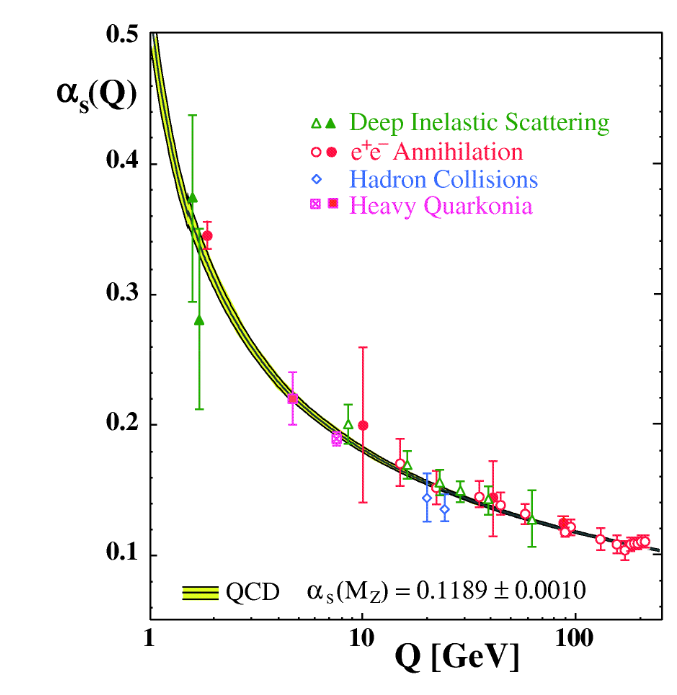
\includegraphics[scale=0.3]{./Obrazky_praca/zrazka.png}
	\caption{Závislosť konštanty silnej interakcie $\alpha_s$ od energetickej škály jednotlivých procesov Q \cite{3}}
	\label{alfa}
\end{figure}

\section{Jety}

Kvarky a gluóny sú uväznené vnútri hadrónov\footnote{Uväznenie kvarkov v hadrónoch je experimenálny fakt, ale na rozdiel od asymptotickej slobody zatiaľ nie je vysvetlené v QCD.}, a teda nemôžeme pozorovať vlastnosti kvarkov a gluónov priamo. Pri udelení dostatočnej energie partónu v hadróne sa táto energia premení na spŕšku hadrónov v jednom smere (tzv. jet), v ktorej sa nachádza hadrón obsahujúci pôvodný partón. V experimentoch je jet definovaný ako skupina energe\-tických hadrónov pohybujúcich sa v jednom smere, ktoré je možné ohraničiť mysleným kužeľom (obr. \ref{jety}) so stredom určeným smerom pohybu originálneho partónu (tzv. jet axis) a s polomerom R~\cite{4}:
\begin{equation}
\sqrt{\Delta \phi^2 + \Delta \eta^2}<R=1,
\end{equation}
kde $\Delta \phi$ je rozdiel azimutálnych uhlov hadrónu v jete a pôvodného partónu, $\Delta \eta$ je rozdiel pseudorapidít\footnote{Pseudorapidita $\eta$ je funkciou polárneho uhla $\theta$: $\eta = - \ln( \tan (\frac{\theta}{2}))$.} hadrónu v jete a pôvodného partónu.
\begin{figure}
	\centering
	\includegraphics[scale=0.6]{./Obrazky_praca/clustering.png}
	\caption{V experimente jety pozorujeme ako spŕšky vysokoenergetických hadrónov v jednom smere, ktoré možno ohraničiť mysleným kužeľom.}
	\label{jety}
\end{figure}

\subsection{Lundský strunový model}
Kým interakcie partónov pri vysokých energiách sú dobre popísané pomocou QCD, na popis vytvárania hadrónov v jetoch si musíme pomôcť fenomenologickými \-mo\-del\-mi. Jeden zo základných modelov, ktorý je prítomný vo väčšine Monte Carlo (MC) generátorov vo fyzike vysokých energií, je Lundský strunový model.

Pre potenciál viazaného stavu kvarku a antikvarku platí:
\begin{equation}
	V(r) \approx - \frac{4}{3} \frac{\alpha_s}{r} + \kappa r \approx - \frac{0.13}{r} + r~\cite{5}
\end{equation}

Na veľmi malých vzdialenostiach ($r\rightarrow0$) prevláda potenciál Coulombovského poľa (obr.~\ref{elpole}). Pri vzájomnom vzďaľovaní sa kvarkov začne prevládať lineárna časť potenciálu a na rozdiel od elekromagnetického poľa sa kvôli samointerakcii gluónov budú siločiary k sebe približovať a vytvoria tvar podobný trubici (obr.~\ref{chrompole}).

Ak je vzdialenosť medzi dvoma kvarkami dostačujúca, z energie poľa sa vytvorí nový pár častíc kvark-antikvark (obr.~\ref{jet}). Takto to pokračuje ďalej, pokiaľ majú vzďaľujúce sa partóny dostatok energie na vytvorenie nového páru kvark-antikvark. Celý proces pripomína trhanie struny, odkiaľ pochádza aj názov modelu.

\begin{figure}[hbtp!]
	\centering
	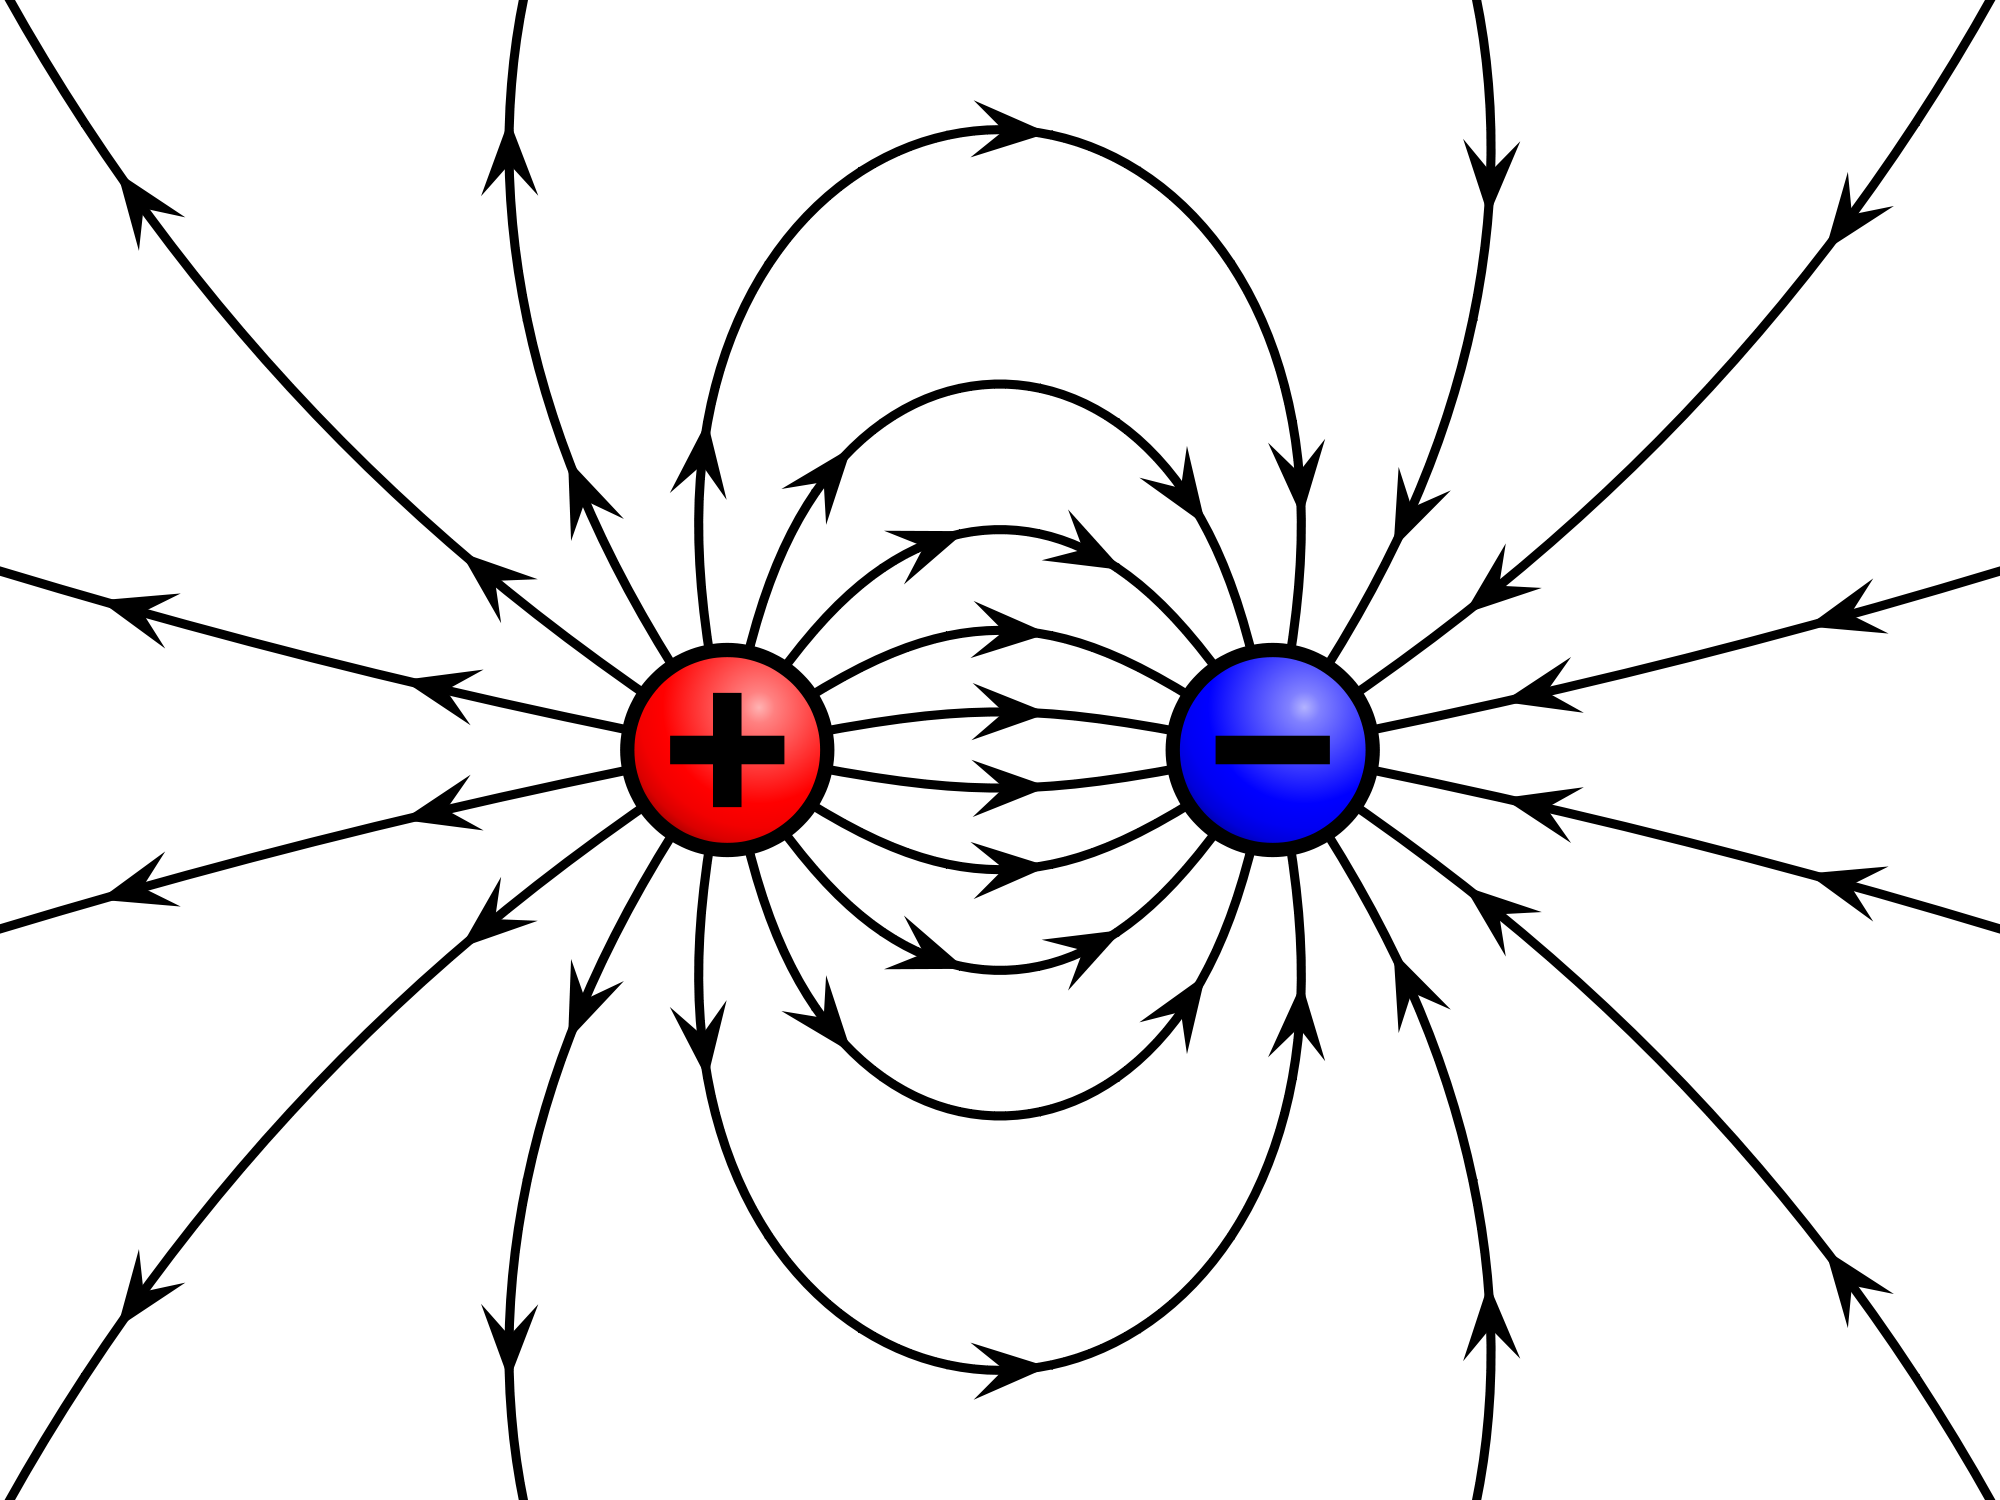
\includegraphics[scale=0.06]{./Obrazky_praca/el_pole.png}
	\caption{Siločiary elektrického poľa sa od seba so zväčšujúcou sa vzdialenosťou vzďaľujú~\cite{6}.}
	\label{elpole}
\end{figure}
\begin{figure}[hbtp!]
	\centering
	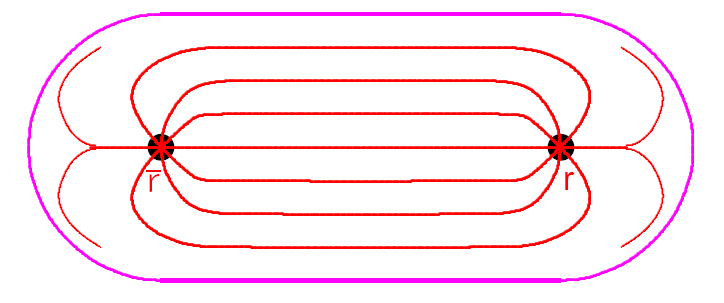
\includegraphics[scale=0.2]{./Obrazky_praca/chromo_pole.png}
	\caption {Siločiary chromodynamického poľa sa k sebe so zväčšujúcou sa vzdialenosťou približujú~\cite{7}.}
	\label{chrompole}
\end{figure}

\begin{figure}[hbtp!]
	\begin{center}
	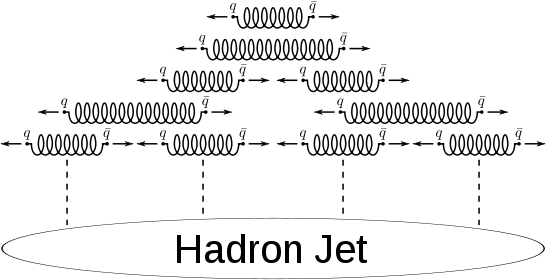
\includegraphics[scale=0.4]{./Obrazky_praca/jet.png}
	\caption{Tvorba jetu pripomína trhanie struny. Čím viac od seba naťahujeme konce struny, tým väčšiu silu musíme vynaložiť. Pri prasknutí struny získame dve nové struny~\cite{8}.}
	\label{jet}
	\end{center}
\end{figure}  


\chapter{Dvojhadrónové korelácie}

\section{Metóda dvojčasticových korelácii}
\label{korel}
Metóda dvojčasticových (dvojhadrónových) korelácii je jednou z nepriamych metód na štúdium jetov. Využíva sa najmä v jadrovo-jadrových zrážkach, kde kvôli \-mo\-di\-fi\-ká\-cii jetov vplyvom QGP nemožno použiť priame metódy, ktoré sú používané pri protónovo-protónových zrážkach.

Spočíva v zvolení intervalu priečnej hybnosti\footnote{Priečna hybnosť je definovaná ako: $p_T=\sqrt{p_x^2+p_y^2}$, pričom rovina $xy$ je kolmá na os zväzku v experimente.}, v ktorom sa hľadá častica s vysokou priečnou hybnosťou, tzv. trigrovacia častica ("trigger particle"), o ktorej sa predpokladá, že je to hadrón obsahujúci pôvodný partón. Tiež je potrebné zvoliť interval nižších hybností pre asociované častice ("\-associated particles"). Následne sa robia rozdiely v \-a\-zi\-mu\-tál\-nom uhle $\phi$ a pseudorapidite $\eta$ pre rôzne intervaly priečnej hybnosti trigrovacích a asociovaných častíc:

\begin{equation}
\Delta \phi = \phi_{trig} - \phi_{asoc}
\end{equation}

\begin{equation}
\Delta \eta = \eta_{trig} - \eta_{asoc}
\end{equation}

Tieto rozdiely sa plnia do dvojrozmerných histogramov, z ktorých sa robia projekcie na jednotlivé osi. V projekcii na $\Delta \phi$ sa vytvoria dva píky zodpovedajúce dvom jetom. Keďže pred zrážkou bola celková priečna hybnosť nulová, vytvorenie jedného jetu je sprevádzané vytvorením jetu na protiľahlej strane v rovine $xy$. Pík  so stredom v 0 sa nazýva priľahlý pík (v angličtine "near-side peak") a je spôsobený pármi, kde asociované častice pochádzajú z toho istého jetu ako trigrovacia častica. Druhý pík sa nachádza v okolí $\pi$ a je spôsobený takými pármi častíc, kde asociovaná častica pochádza z jetu, ktorý je oproti jetu, z ktorého je trigrovacia častica. Preto sa nazýva protiľahlý pík (v angličtine ''away-side peak'')(obr.~\ref{kor}). Iná situácia nastáva v pozdĺžnom smere. Partóny v protónoch vo zväzku môžu mať v princípe rôznu pozdĺžnu hybnosť, a teda, ak vidíme v detektore jet v pozdĺžnom smere, druhý nemusí byť na protiľahlej strane. Výberom trigrovacej častice vyberáme jety, ktoré sa nachádzajú v detektore a ich náprotivky sa nemusia nachádzať v skúmanom intervale $\Delta \eta$.

\begin{figure}[hbtp!]
	\begin{center}
		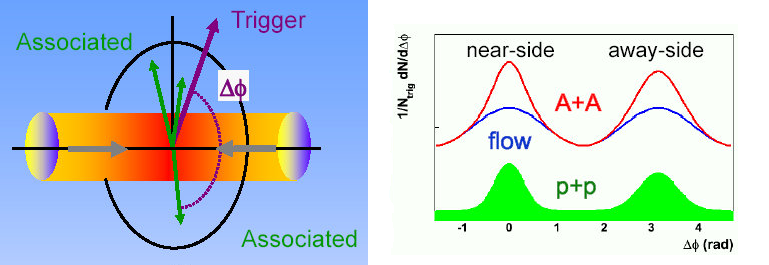
\includegraphics[width=\textwidth]{./Obrazky_praca/dijetcorrelations.png}
		\caption{Vľavo: Schéma polohy trigrovacej a asociovanej častice. Vpravo: Poloha priľahlého a protiľahlého píku pre protónovo-protónové a jadrovo-jadrové zrážky. Pozadie v protónovo-protónových zrážkach je konštantné, v jadrovo-jadrových zrážkach je \-mo\-di\-fi\-ko\-va\-né kolektívnym tokom (flow).}
		\label{kor}
	\end{center}
\end{figure}

Po korekciách na akceptanciu detektora a na účinnosť rekonštrukcie dráh asociovaných a trigrovacích častíc, po normovaní na počet trigrovacích častíc a po odpočítaní pozadia, ktoré je v prípade protónovo-protónových zrážok konštantné a v prípade jadrovo-jadrových zrážok modifikované kolektívnym tokom, sa počítajú výťažky \-"yields" \- - pre jednotlivé intervaly priečnej hybnosti trigrovacích častíc. Výťažky, ktoré predstavujú priemerný počet asociovaných častíc na jednu trigrovaciu časticu pri danej priečnej hybnosti, možno vypočítať ako:

\begin{equation}
Y_J^{\Delta\phi}=\int_{\Delta \phi_1}^{\Delta \phi_2} \frac{dN}{d\Delta \phi } d\Delta\phi 
\label{yield}
\end{equation} 

\section{Doterajšie výsledky pre pp a PbPb zrážky}
\label{ALICEPbPb}
QGP, ktorá vzniká v zrážkach relativistických ťažkých iónov, je študovaná pomocou signatúr spojených s produkciou a vlastnosťami rôznych častíc. Jednou z týchto signatúr je modifikácia jetov vplyvom QGP. Jety s istými energiami dokonca nie sú v dátovej vzorke prítomné, pretože boli absorbované plazmou. Tento jav sa nazýva "jet quenching" (z angl. - zhášanie jetov) a bol prvýkrát pozorovaný pri štúdiu dvoj\-čas\-ti\-co\-vých korelácii pri zrážkach zlato-zlato pri energii $\sqrt{s_{NN}}=$130 GeV na urýchľovači RHIC~\cite{rhic}.

V kolaborácii ALICE bolo analyzovaných 14 miliónov oloveno-olovených zrážok z roku 2010 pri energii $\sqrt{s_{NN}}=$ 2.76 TeV a 37 miliónov protónovo-protónových zrážok z marca 2011 pri rovnakej energii metódou dvojčasticových korelácií. Dáta boli analyzované pre intervaly $8<p^{trig}_{T}<15$ GeV/$c$ a 3 GeV/$c<p^{assoc}_{T}<p_T^{trig}$ a merali sa pomery výťažkov v centrálnych zrážkach ku výťažkom v periférnych zrážkach ($I_{CP}$) a pomery výťažkov v oloveno-olovených ku protónovo-protónovým zrážkam ($I_{AA}$) pre rôzne centrality \cite{clanok}. Pomer $I_{AA}$ ukazuje vplyv plazmy na konečné stavy hadrónov. 

Na obrázku~\ref{clanok2} sú zobrazené pomery $I_{AA}$ pre centrálne a periférne zrážky, pričom boli použité tri spôsoby odčítania pozadia. Potlačenie výťažku $I_{AA}\approx0.6$ pre protiľahlý pík centrálnych zrážok je považované za dôkaz straty energie v QGP. Viditeľné je aj zvýšenie pre priľahlý pík, $20-30\%$, ktoré nebolo pozorované pri nižších energiách zrážok na RHICu. Pre periférne zrážky nie sú zreteľné žiadne vplyvy plazmy, ako bolo očákavané. Podľa výsledkov tejto analýzy je pomer $I_{CP}$ v súlade s $I_{AA}$ pre centrálne zrážky (obr.~\ref{clanok2}).

Počas tejto analýzy bolo prvý krát pozorované už skôr spomenuté navýšenie pomeru $I_{AA}$ pre centrálne zrážky, čo napovedá, že aj priľahlý partón bol ovplyvnený QGP. V publikácii~\cite{clanok} sú uvedené 3 faktory ovplyvňujúce toto navýšenie:
\begin{itemize}
	\item \textbf{zmena fragmentačnej funkcie\footnote{Fragmentačná funkcia vo všeobecnosti popisuje transformáciu farebne nabitých kvarkov a gluónov na bezfarebné hadróny a fotóny.}}: vplyvom plazmy nesú hadróny v oloveno-olovených zrážkach menšiu časť hybnosti pôvodného partónu ako v protónových zrážkach, čo vedie k zvýšenému počtu asociovaných častíc a $I_{AA}>1$
	\item \textbf{rôzna distribúcia počiatočných partónov}: zvýšený počet gluónov má rovnaký vplyv a vedie k potlačeniu počtu trigrovacích častíc v danom $p_T$ intervale, z čoho plynie $I_{AA}>1$
	\item \textbf{posun $p_T$ spektra partónu}: pre danú $p_T$ trigrovacej častice, mal pôvodný partón vyššiu $p_T$ v oloveno-olovených zrážkach ako v protónovo-protónových, čo vedie k zvýšeniu $I_{AA}$
\end{itemize}

Predpokladá sa, že všetky tri efekty hrajú úlohu a prispievajú k nameranému výsledku.

\begin{figure}[hbtp!]
	\centering
	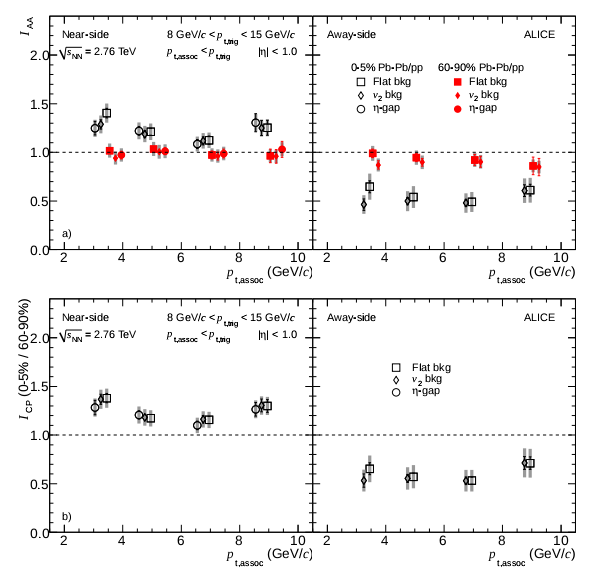
\includegraphics[scale=0.8]{./Obrazky_praca/clanok2.png}
	\caption{ Hore: $I_{AA}$ pre centrálne a periférne zrážky; dole: $I_{CP}$: Výsledky získané pomocou rôznych metód odčítania pozadia~\cite{clanok}}
	\label{clanok2}
\end{figure}

V doterajších výsledkoch štúdia protónovo-protónových zrážok pri energii $\sqrt{s_{NN}}=$7 TeV a protónovo-olovených zrážok pri energii $\sqrt{s_{NN}}=$5,02 TeV boli pozorované niektoré znaky kvarkovo-gluónovej plazmy vo vysokomultiplicitých zrážkach. Jedným z nich je zvýšená produkcia podivnosti pozorovaná v analýze \cite{nature}. Ďalším sú znaky kolektívneho toku pozorované pri analýze pomocou dvojčasticových korelácií \cite{AlicepPb}. Preto by bolo zaujímavé študovať protónovo-protónové zrážky pomocou h-h\footnote{Korelácie medzi dvoma nabitými hadrónmi.}  korelácií pri ešte vyšších energiách, $\sqrt{s_{NN}}=$13 TeV, v závislosti od multiplicity zrážky.

\chapter{Ciele práce} 
\begin{itemize}
	\item Skúmanie jetov vzniknutých v pp zrážkach pri 13 TeV prostedníctvom h-h korelácií
	\begin{itemize}
		\item Vypracovanie analyzačného programu
		\item Analýza dát pp pri 13 TeV
		\item Analýza MC simulácií
		\begin{itemize}
			\item Výpočet účinnosti rekonštrukcie asociovaných častíc
			\item Výpočet účinnosti rekonštrukcie trigrovacích častíc
			\item Vypracovanie MC closure testu
		\end{itemize}
		\item Štúdium niektorých zdrojov systematických chýb
		\item Výpočet výťažkov v závislosti od multiplicity zrážky a od priečnej hybnosti trigrovacej častice
	\end{itemize}
\end{itemize}


\chapter{Metóda merania}

\section{Experiment ALICE}

ALICE (z anglického A Large Ion Collider Experiment – experiment na Veľkom iónovom zrážači) je jedným zo štyroch veľkých experimentov na LHC v CERNe. Zameriava sa najmä na výskum partónovej hmoty vznikajúcej v zrážkach ultrarelativistických ťažkých iónov. Táto hmota sa svojimi vlastnosťami podobá na teoreticky predpovedanú QGP, ktorou bol tvorený Vesmír tesne po Veľkom Tresku. V podmienkach LHC to zodpovedá približne 1 miliardtine sekundy veku Vesmíru.

Detektor  ALICE umožňuje detekciu rôznych druhov častíc pri zrážkach protón - protón, ale predovšetkým umožňuje štúdium zrážok olovo - olovo pri extrémnych podmienkach (vysoká teplota, tlak a energia). Jeho rozmery dosahujú $16\times 16\times26 \rm{m^3}$ s váhou približne 10,000 ton~\cite{alice}. Valcová časť detektora je umiestnená v solenoidálnom magnetickom poli s indukciou 0.5 T, ktoré spôsobuje zakrivenie dráh a umožňuje tak určenie hybnosti a elektrického náboja jednotlivých častíc.

Experiment ALICE je tvorený viacerými detektormi, ako je zobrazené na obrázku \ref{ALICE}. Každý z jednotlivých subdetektorov využíva inú technológiu a má svoju nezastupiteľnú úlohu v celom detektorovom komplexe. Pri analýze dvojhadrónových korelácií hrajú nezastupiteľnú úlohu detektory ITS, V0 a TPC.

\begin{figure}[hbtp!]
	\begin{center}
		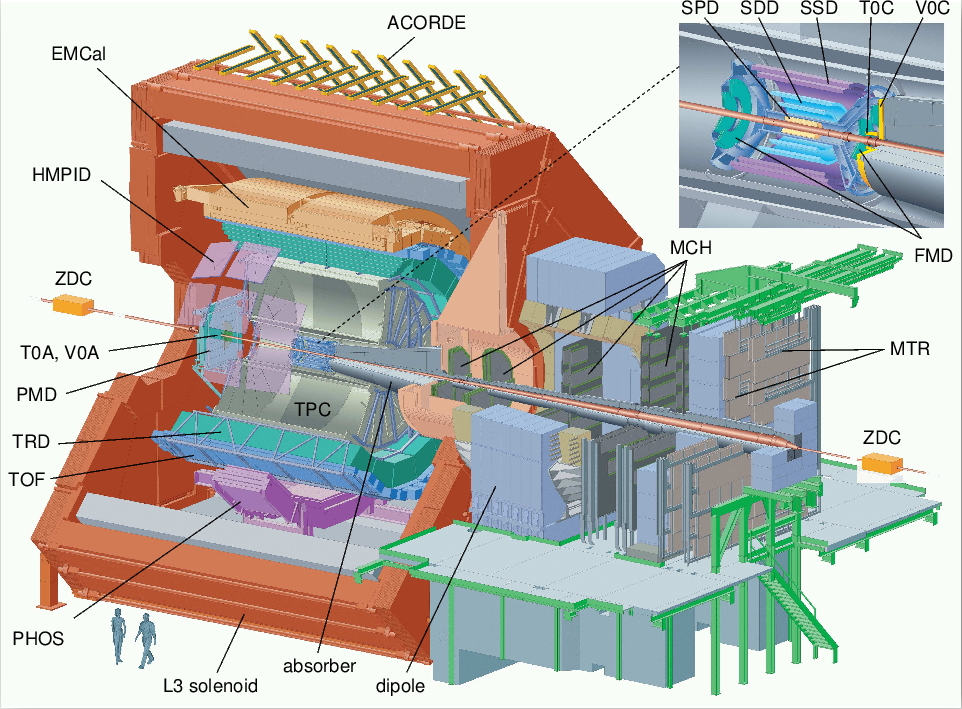
\includegraphics[width=0.9\textwidth]{./Obrazky_praca/ALICE.png}
		\caption{Experiment ALICE skladajúci sa z viacerých subdetektorov~\cite{aliceDetektor}}
		\label{ALICE}
	\end{center}
\end{figure}

\subsection{Vnútorný dráhový systém}

ITS (z anglického Inner Tracking System) je systém najvnútornejších detektorov, ktorý sa nachádza blízko miesta zrážky, a teda v oblasti s vysokou hustotou častíc (pre zrážky olovo-olovo až 50 dráh na $\mathrm{cm}^2$ ). Je tvorený šiestimi vrstvami kremíkových detektorov, ktoré slúžia najmä na detekciu primárneho vertexu (PV)\footnote{Miesto, kde nastala zrážka.}, určovanie sekundárneho vertexu slabých rozpadov a určovanie a rozlišovanie dráh jednotlivých častíc. Pokrýva peudorapiditný interval $|\eta|<$0,9.

\subsection{V0 detektor}

 V0 je tvorený dvoma kruhovými časťami (V0A a V0C), pričom každá z nich sa náchadza na jednej strane ITS. Každý z kruhov je tvorený 32 scintilačnými detektormi. V0 detektory pokrývajú preudorapiditné intervaly $2,8 <\eta<5,1$ (V0A) a $-3,7<\eta<-1,7$ (V0C). Jeho hlavnou úlohou je "triggering"\footnote{Trigger je elektronický systém, ktorý na základe signálov z detektorov rozhoduje, či došlo k fyzikálne zaujímavej zrážke, ktorá bude uložená na grid a následne spracovávaná.} pre centrálne barelové detektory a vďaka monotónnej závislosti počtu detekovaných častíc od počtu primárne emitovaných častíc v zrážke je užitočným detektorom na určovanie centrality\footnote{Miera prekryvu jadier pri oloveno-olovených zrážkach.} zrážok pomocou určovania multiplicity\footnote{Multiplicita je stredná hodnota hustoty primárnych nabitých častíc v strednej pseudorapidite   \newline  ($\braket{dN_{ch}/d\eta}_{|\eta|<0.5}$).} zrážok.  

\subsection{Časovo-projekčná komora}
\label{textTPC}
Na pozorovanie dráh nabitých častíc produkovaných v zrážkach slúžia dráhové detektory. Hlavný z nich je TPC (z anglického Time Projection Chamber - časovo projekčná komora).

TPC je valec naplnený plynovou zmesou ( $Ne/CO_2/N_2$) s objemom 88 m$^3$ (obr.~\ref{tpc}) rozdelený centrálnou elektródou na dve driftovacie časti. Pozdĺž z-ovej osi je udržiavané rovnomerné elektrické pole o veľkosti 100kV. Nabité častice pri svojej ceste ionizujú plyn v TPC. Tým sú uvoľňované elektróny z molekúl plynu, ktoré po krátkom vychýlení následne driftujú k anódam na okraji valca. Na základe informácie o čase driftu elektrónov a o mieste ich dopadu sa rekonštruujú body v priestore, cez ktoré častica preletela. Signál je zosilnený lavínovým efektom v blízkosti anódy~\cite{TPCobr}, ktorá je tvorená mnohovláknovými proporcionálnymi komorami. Tie sú rozdelené na 18 sektorov v azimutálnom uhle a na 2 sektory v radiálnom smere. Homogénne magnetické pole v smere osi z, v ktorom je celý detektor umiestnený, umožňuje určenie hybnosti a elektrického náboja častíc. Z informácií o energetických stratách v TPC a v iných detektoroch je možné určiť aj druh častice. 

\begin{figure}[hbtp!]
	\begin{center}
	 	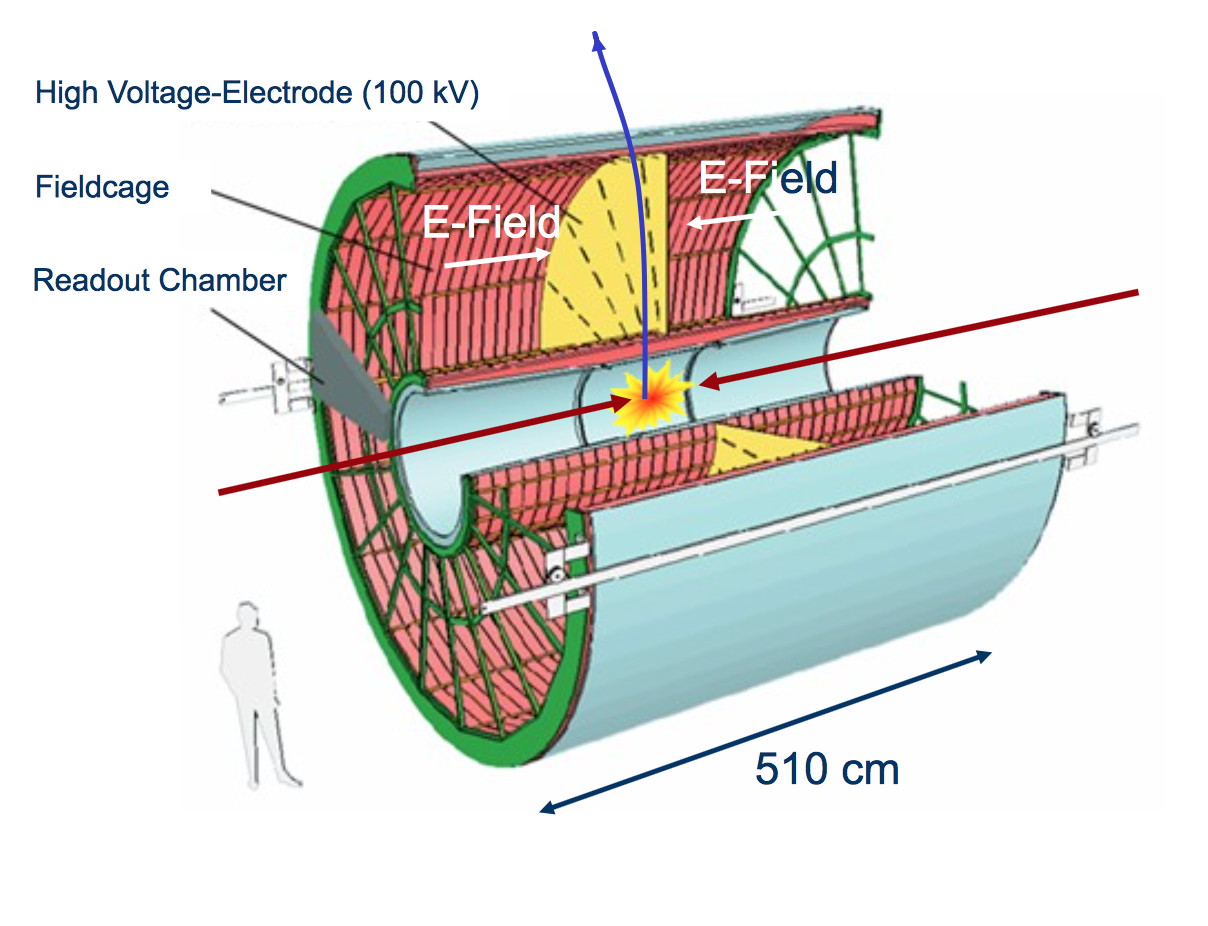
\includegraphics[width=0.7\textwidth]{./Obrazky_praca/tpc.png}
		\caption{Porovnanie veľkosti TPC s veľkosťou človeka~\cite{TPCobr}.}
		\label{tpc}
	\end{center}
\end{figure}

\section{ROOT}
ROOT je vývojové prostredie napísané v objektovo orientovanom programovacom jazyku C++ určené na analýzu dát. Užívateľovi poskytuje veľký počet funkcionalít spojených so spracovávaním veľkého množstva dát, napr. histogramy, funkcie pre štatistickú analýzu, vizualizáciu zrážok a bohatý matematický aparát. Užívateľ má taktiež možnosť vytvorenia vlastných tried a knižníc vhodných pre svoju analýzu. ROOT je možné prepojiť s už existujúcimi programovacími jazykmi a štatistickými programami, ako sú Python, Ruby, R a Mathematica~\cite{root}.

\section{AliRoot}
AliRoot \cite{aliroot} je oficiálnym analyzačným softvérom kolaborácie ALICE, základom kto\-ré\-ho je ROOT rozšírený o špeciálne triedy, ktoré sa používajú na rekonštrukciu, simuláciu a analýzu dát v experimente ALICE. Jeho štruktúra, triedy a funkcie sú vytvárané v súlade s~potrebami analýzy dát nameraných na experimente ALICE. Z toho vyplýva aj delenie jeho tried na všeobecné a triedy využívané pri rekonštrukcii, simulácii a analýze. 



\section{Spracované dáta a selekčné kritéria}
V analýze boli spracovávané dáta z protónovo-protónových zrážok pri energii $\sqrt{s_{NN}}=13$~TeV z roku 2015. Dokopy bolo analyzovaných $1.17\times10^7$ zrážok, ktoré boli vyselektované na základe tzv. minimum bias triggera, ktorý bol definovaný ako koincidencia medzi signálmi z detektorov V0A a V0C.
Bola použitá MC produkcia PYTHIA6 - Perugia \cite{perugia}, ktorá je zviazaná s týmito dátami\footnote{Podmienky, pri ktorých boli zbierané dáta, boli implementované aj do nastavení simulácie. } . 

Analyzované boli iba tie zrážky, ktorých PV bol vzdialený maximálne 10 cm od geometrického stredu detektora. Nabité primárne hadróny museli spĺňať základné detektorové selekčné kritériá pre TPC a ITS. 

Posledným kritériom potrebným na štúdium dvojčasticových korelácií je priečna hybnosť. Trigrovacia častica musela mať priečnu hybnosť väčšiu ako 4 GeV/$c$ a asociovaná sa musela nachádzať v intervale 2 GeV/$c<p_T^{asoc}<p_T^{trig}$.

\section{Korekcie}
Okrem jednotlivých selekčných kritérii bolo potrebné pri analýze použiť aj tri korekcie. 

Prvou je korekcia na konečnú akceptanciu detektora. Túto korekciu sme urobili pomocou metódy mixing. Trigrovacia častica bola z jedného prípadu a asociovaná častica z iného nezávislého prípadu. Kvôli väčšej štatistike sme jednu trigrovaciu časticu mixovali s minimálne piatimi prípadmi, pričom oba prípady museli mať z-ovú zložku primárneho vertexu rovnakú v rámci 1 cm a mať približne rovnakú multiplicitu. Mixovaním získané rozdelenie tvaru kombinatorického pozadia v rovine ($\Delta \phi, \Delta \eta$) je na obrázku~\ref{pozadie}. Toto rozdelenie bolo následne normované na hodnotu najvyššieho binu rozdelenia ($\beta$). Za predpokladu, že účinnosť rekonštrukcie páru v najvyššom bine je 100\%, získame tak rozdelenie účinnosti rekonštrukcie párov v priestore $(\Delta \phi,\Delta\eta)$.

\begin{equation}
	\epsilon_{pair}(\Delta\phi,\Delta\eta) = \frac{d^2N^{mixed}_{pair}}{d\Delta\phi d\Delta\eta}\frac{1}{\beta}
\end{equation}

\begin{figure}[hbtp!]
	\centering
	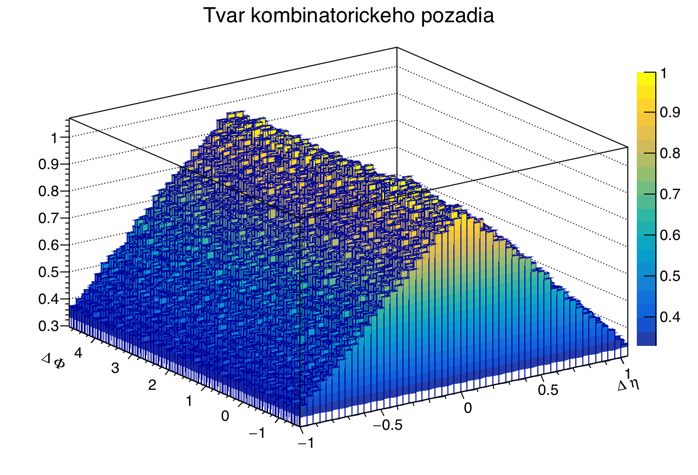
\includegraphics[scale=0.5]{./Obrazky_praca/pozadie.png}
	\caption{Príklad tvaru kombinatorického pozadia, t.j. častice v páre spolu fyzikálne nesúvisia, pri dvojčasticových koreláciách namodelovaného metódou mixing}
	\label{pozadie}
\end{figure}

Druhou je korekcia na účinnosť rekonštrukcie asociovaných častíc v detektore. Pri tejto korekcii boli použité dáta nasimulované metódou Monte Carlo (MC), ktoré zodpovedajú energii aj druhu zrážok spracovávaných dát. Generované dáta prešli re\-kon\-štruk\-ciou, pri ktorej boli použité rovnaké selekčné kritéria ako pre reálne dáta. Účinnosť re\-kon\-štruk\-cie sa definuje ako podiel počtu zrekonštruovaných častíc ku počtu generovaných častíc, pričom každá rekonštruovaná častica musí byť prepojená s generovanou časticou, t.j. nebolo možné zrekonštruovať časticu, ktorá nebola pre danú zrážku vygenerovaná. Účinnosť rekoštrukcie sme skúmali v závislosti od $p_T$, $\eta$ a polohy PV (obr. ~\ref{uc}). Korekciu na účinnosť v závislosti od z-ovej súradnice primárneho vertexu sme ale nebrali do úvahy, pretože ako je vidieť na obr. \ref{ucpvz}, účinnosť je vzhľadom na polohu PV konštantná.    
\begin{equation}
\epsilon_{asoc}(p_{T}^{asoc},\eta^{asoc}) = \frac{N_{asoc}^{rek}}{N_{asoc}^{gen}}(p_{T}^{asoc},\eta^{asoc})
\end{equation}
Poslednou je korekcia na účinnosť rekonštrukcie trigrovacích častíc\footnote{Takáto korekcia na účinnosť rekonštrukce trigrovacích častíc bola robená aj v predchádzajúcich korelačných analýzach \cite{Jan-Fiete}.}. Bola robená podobne ako pre asociované častice v závislosti od priečnej hybnosti a pseudorapidity trigrovacej častice.  
\begin{equation}
\footnotesize
\epsilon_{trig}(p_{T}^{trig},\eta^{trig}) = \frac{N_{trig}^{rek}}{N_{trig}^{gen}}(p_{T}^{trig},\eta^{trig})
\end{equation}
\begin{equation}\end{equation}


\begin{figure}[hbtp!]
	\centering
	\begin{subfigure}{0.33\textwidth}
		\centering
		\includegraphics[width=1.\linewidth]{./Obrazky_praca/eff_pt.png}
		\caption{}
		\label{}
	\end{subfigure}%
	\begin{subfigure}{0.33\textwidth}
		\centering
		\includegraphics[width=1.\linewidth]{./Obrazky_praca/eff_eta.png}
		\caption{}
		\label{}
	\end{subfigure}
\begin{subfigure}{0.33\textwidth}
	\centering
	\includegraphics[width=1.\linewidth]{./Obrazky_praca/eff_pvz.png}
	\caption{}
	\label{ucpvz}
\end{subfigure}
	\caption{Účinnosť rekonštrukcie nabitých hadrónov v závislosti od ich priečnej hybnosti (a) , pseudorapidity (b) a z-ovej zložky polohy PV (c).}
	\label{uc}
\end{figure}

\section{MC closure test}

Monte Carlo closure test je v princípe skúška správnosti kódu použitého na štúdium dvojčasticových korelácií. V rámci tohto testu sa pozeráme na korelačné \-funk\-cie hadrónov, ktoré boli vygenerované a na korelačné funkcie MC zrekonštruovaných hadrónov, na ktoré boli aplikované už skôr spomínané korekcie. Pre generované ako aj rekonštruované dáta sme urobili korelačné funkcie v závislosti od priečnej hybnosti. Následne sme dvojrozmerné rozdelenia generovaných častíc predelili rozdeleniami rekonštruovaných častíc. Z týchto dvojrozmerných pomerov sme potom vytvorili projekcie na jednotlivé osi, pričom prázdne biny boli ignorované, a tie sme fitovali konštantnou funkciou. Hodnoty jednotlivých fitov sme zobrazili v závislosti od priečnej hybnosti (obr. \ref{fitMC}) . 

Ak boli všetky použité korekcie správne a dostatočne presné, výsledok by sa mal nachádzať v blízkom okolí 1, ktorý sme aj dosiahli  (obr.\ref{hphi} a obr.\ref{heta}). Tento výsledok znamená, že sa nám podarilo dostatočne dobre popísať vplyv detektora.  

\begin{figure}
	\centering
	\begin{subfigure}{0.5\textwidth}
		\centering
		\includegraphics[width=1.1\linewidth]{../histogramy/PorovnanieMC/Projekcie/fitPhiHH.png}
		\caption{}
		\label{fitPhi}
	\end{subfigure}%
	\begin{subfigure}{0.5\textwidth}
		\centering
		\includegraphics[width=1.1\linewidth]{../histogramy/PorovnanieMC/Projekcie/fitEtaHH.png}
		\caption{}
		\label{fitEta}
	\end{subfigure}
	\caption{Hodnota fitu pre jednotlivé $p_{T}^{trig}$ biny.}
	\label{fitMC}
\end{figure}

\begin{figure}
	\centering
	\includegraphics[width=1\linewidth]{../histogramy/PorovnanieMC/Projekcie/15a+c_hh_phi.png}
	\caption{Generované/rekonštruované - projekcia na os $\Delta \phi$ }
	\label{hphi}
\end{figure}

\begin{figure}
	\centering
	\includegraphics[width=1\linewidth]{../histogramy/PorovnanieMC/Projekcie/15a+c_hh_eta.png}
	\caption{Generované/rekonštruované - projekcia na os $\Delta \eta$ }
	\label{heta}
\end{figure}

\chapter{Výsledky}
 Po aplikovaní všetkých korekcií dostávame výsledné dvojrozmerné rozdelenie, ktoré ešte normujeme na počet trigrovacích častíc:
\begin{equation}
\footnotesize
\frac{d^2N^{corrected}_{pair}}{d\Delta\phi d\Delta\eta}(\Delta\phi,\Delta \eta)=
\frac{1}{N^{corr}_{trig}} \frac{d^2N^{raw}_{pair}}{d\Delta\phi d\Delta\eta} \frac{1}{\epsilon_{asoc}(p_{T}^{asoc},\eta^{asoc})}\frac{1}{\epsilon_{pair}(\Delta\phi,\Delta\eta)}
\frac{1}{\epsilon_{trig}(p_{T}^{trig},\eta^{trig})}
\label{korfunc}
\end{equation}
\begin{equation}
\footnotesize
N^{corr}_{trig}=N^{raw}_{trig}\frac{1}{\epsilon_{trig}(p_{T}^{trig},\eta^{trig})}
\end{equation}

Aby sme mohli sledovať závislosť výťažkov od multiplicity, zrážky sme rozdelili na 3 kategórie: 0-10\% - zrážky s najvyššou multiplicitou (viac ako 11,5 $\braket{dN_{ch}/d\eta}$), 10-50\% - zrážky so strednou multiplicitou (4,5 - 11,5 $\braket{dN_{ch}/d\eta}$) a 50-100\% - zrážky s nízkou multiplicitou (menej ako 4,5 $\braket{dN_{ch}/d\eta}$).
Na získanie výťažkov sme najprv z dvojrozmerného korigovaného rozdelenia $\frac{d^2N}{d\Delta \phi d\Delta \eta}$ (vzťah \ref{korfunc}), ktoré bolo podelené rozdelením získaným z metódy mixing a korigované na efektivitu rekonštrukcie asociovaných aj trigrovacích častíc, projektovali jednorozmerné histogra\-my pozdĺž osi $\Delta\phi$ v jednotlivých multiplicitných binoch pre rôzne intervaly priečnej hybnosti trigrovacej častice. Jednorozmerné rozdelenia sme následne normovali na počet trigrovacích častíc, ktoré boli taktiež korigované na efektivitu rekonštrukcie trigrovacích častíc. 

Pozadie sme určovali pomocou konštantnej funkcie. Jej hodnota bola vypočítaná ako aritmetický priemer hodnoty rozdelenia v troch binoch okolo 1 a troch binoch okolo $-1$. Rozdelenia po odčítaní pozadia takouto metódou sú zobrazené na obr. \ref{dphi}.

\begin{figure}
	\centering
	\includegraphics[width=1\linewidth]{./Obrazky_praca/hhDeltaPhi.png}
	\caption{Rozdelenie $\Delta \phi$ pre nabitý hadrón ako trigrovaciu časticu po odčítaní pozadia pre rôzne intervaly $p_T^{trig}$}
	\label{dphi}
\end{figure}

Výťažky sme počítali pomocou vzťahu~\ref{yield} v intevale $-0.9$ až 0.9 pre priľahlý pík a v intervale $\pi\pm1.5$ pre protiľahlý pík. Výťažky v závislosti od priečnej hybnosti trigrovacej častice a multiplicity zrážky sú zobrazené na obr.  \ref{hhmult}. Na tomto grafe sú zobrazené aj výťažky pre "minimum bias" zrážky, v našom prípade to znamená zrážky vo všetkých multiplicitných binoch. Pozorujeme motónny nárast výťažkov s narastajúcou $p_{T}^{trig}$.

\begin{figure}
	\centering
		\includegraphics[width=0.8\linewidth]{./Obrazky_praca/vytazky_hh_prilahly_mult.png}
		\caption{}
		\label{hhpril}
	\caption{Závislosť výťažkov pre korelácie $h - h$ od $p_T^{trig}$ a multiplicitnej triedy zrážky pre priľahlý pík. Štatistická chyba je znázornená čiarami a systematická obdlížnikmi.}
	\label{hhmult}
\end{figure}

\begin{figure}
	\centering
	\includegraphics[width=0.8\linewidth]{./Obrazky_praca/vytazky_hh_protilahly_mult.png}
	\caption{}
	\label{hhproti}
	\caption{Závislosť výťažkov pre korelácie $h - h$ od $p_T^{trig}$ a multiplicitnej triedy zrážky pre protiľahlý pík. Štatistická chyba je znázornená čiarami a systematická obdlížnikmi.}
\end{figure}

Podobne, ako bolo relizované v skoršej analýze na experimente ALICE \cite{AlicepPb}, skúsili sme porovnať dvojrozmerné korelačné funkcie pre jednotlivé multiplicitné triedy zrážok. Na obr. \ref{multroz} je zobrazený rozdiel korelačných funkcií pre triedu najvyšších a najnižších multiplicitných tried ((0-10\%)-(50-100\%)). Vidíme jasný pík v okolí bodu (0,0) a žiadne navýšenie v okolí bodov s $\Delta\phi \approx \pi$.

Tento efekt sa dá kvalitatívne zobraziť ako na obr. \ref{Icpnase}, kde sme porovnali veľkosti výťažkov pre zrážky s najvyššou a najnižšou multiplicitou. Vypočítali sme pomer $I_{CP}$,  teda delili sme  výťažky vysokomultiplicitých zrážok výťažkami  z nízkomultiplicitných zrážok. Tento pomer sme počítali v závislosti od priečnej hybnosti trigrovacej častice pre priľahlý aj protiľahlý pík. Vidíme navýšenie pre priľahlý pík a náznak mierneho potlačenia pre protiľahlý pík pre vysoké $p_T^{trig}$. 

\begin{figure}[hbtp!]
	\centering
	\includegraphics[width=0.8\textwidth]{./Obrazky_praca/odcitane.png}
	\caption{Rozdiel korelačných funkcií pre (0-10\%)a (50-100\%) pre všetky $p_T^{trig}$.}
	\label{multroz}
\end{figure}

\begin{figure}[hbtp!]
	\centering
	\includegraphics[width=0.8\textwidth]{./Obrazky_praca/ICPhh.png}
	\caption{Podiel výťažkov vysokomultiplicitých a nízkomultiplicitných zrážok v závislosti od $p_{T}^{trig}$. Štatistická chyba je znázornená čiarami a systematická obdlížnikmi.}
	\label{Icpnase}
\end{figure}
\chapter{Diskusia}
 
Na grafoch závislosti výťažkov od priečnej hybnosti trigrovacej častice je viditieľné, že výťažok rastie so zväčšujúcou sa $p_T$ trigrovacej častice pre priľahlý aj pre protiľahlý pík pre všetky multiplicity. Tento výsledok bol očákavaný, pretože trigrovacia častica s vysokou $p_T$ pochádza z jetu s vysokou energiou, ktoré majú vyššiu multiplicitu ako jety s nižšou energiou, a teda sa tam nachádza väčší počet asociovaných častíc. 

Výťažky protiľahlých píkov sú nižšie ako priľahlých. Tento efekt môže byť spô\-so\-be\-ný tým, že protiľahlý jet nie je viditeľný v detektore v prípade, že sa nachádza v intervale pseudorapidity mimo akceptancie detektora. 

Závislosť výťažkov od multiplicitnej triedy zrážky je jasne viditeľná. Navyššie výťažky pre priľahlý pík sú pozorované pre zrážky s najvyššou multiplicitou a najnižšie pre zrážky s najnižsou multiplicitou.  Pre protiľahlé píky pre vysoké priečne hybnosti trigrovacích častíc je viditeľný opačný efekt, t.j. najvyšší výťažok majú zrážky s najnižšou multiplicitou.  
  
Skúmali sme aj štruktúru dvojrozmernej funkcie, ktorá vznikla odčítaním 2D funkcie pre nízkomultiplicitné zrážky od 2D funk\-cie pre vysokomultiplicitné zrážky pre korelácie s nabitým hadrónom. Z obr. \ref{multroz} je zrejmé, že na rozdiel od analýzy \cite{AlicepPb} sme v našej anlaýze žiadne štruktúry pripomínajúce oloveno-olovené zrážky nepozorovali. Hlavným dôvodom by mohlo byť to, že v našej nalýze sme sa zamerali len na tvrdé nepružné procesy, t.j. skúmali sme len častice s relatívne vysokou priečnou hybnosťou ($p_{T}^{trig}>4$ GeV/$c$), zatiaľ čo v analýze \cite{AlicepPb} sa zameriavali na častice s nižšou priečnou hybnoťou a tým pádom na mäkkšie procesy. 

Na tom istom obrázku je ďalej viditeľné, že aj po odčítaní funkcie pre níz\-ko\-mul\-tip\-li\-cit\-né zrážky zostal korelačný pík v okolí bodu 0,0. Z toho vyplýva, že nárast výťažkov s multiplicitou v našej analýze je spôsobený nárastom korelačného píku (vyššia multiplicita v jetoch) a nie javom, ktorý pripomína kolektívny tok ako v \cite{AlicepPb}.

Z pomeru $I_{CP}$ (obr. \ref{Icpnase}) je viditeľné približne 20\% navýšenie výťažku pre priľahlý a 10\% potlačenie pre protiľahlý pík pre korelácie s nabitým hadrónom, pričom podobný efekt bol nameraný v analýze opísanej v sekcii \ref{ALICEPbPb}, kde bol vysvetlený prí\-tom\-nos\-ťou kvarkovo-gluónovej plazmy, pretože sa jednalo o oloveno-olovené zrážky. V tejto práci však boli analyzované protónovo-protónové zrážky, kde doteraz prítomnosť kvarkovo-gluónovej plazmy nebola potvrdená.

\section{Štúdium niektorých zdrojov systematických chýb}

\begin{figure}[hbtp!]
	\centering
	\includegraphics[width=0.8\textwidth]{./Obrazky_praca/neistotaHH.png}
	\caption{Veľkosti systematických chýb z jednotlivých zdrojov a celková relatívna systematická neistota merania výťažkov pre priľahlý a protiľahlý pík.}
	\label{systchyba}
\end{figure}

Pre krátkosť času nebolo možné v tejto analýze študovať všetky zdroje systematických chýb, ale vybrali sme len tie, ktoré najviac ovplyvňujú výpočet výťažkov z korelačnej analýzy.

Prvá chyba pochádza z metódy mixing, konkrétne zo spôsobu, ako bola určená 100\% účinnosť rekonštrukcie páru. V analýze sme predpokladali, že 100\% účinnosť je v najvyššom bine 2D rozdelenia kombinatorického pozadia. Pri výpočte systematickej chyby sme za 100\% účinnosť zobrali aritmetický priemer všetkých binov so súradnicou $\Delta\eta=0$. S takto naškálovaným kombinatorickým pozadím sme vypočítali výťažky a následne aj absolútnu systematickú chybu z tohto zdroja, ktorá je definovaná ako rozdiel výťažkov vypočítaných v rámci analýzy a výťažkov vypočítaných pomocou inak naškálovaného kombinatorického pozadia. Relatívnu systematickú chybu sme dostali podelením absolútnej chyby výťažkom v danom $p_T$ bine.

Druhým študovaným zdrojom bola metóda odčítania pozadia z jednorozmerného rozdelenia $\Delta\phi$ pred výpočtom výťažkov. V analýze sme za pozadie pokladali konštantnú funkciu, ktorej hodnotu sme vypočítali ako aritmetický priemer šiestich binov mimo píkov. Pri výpočte systematickej chyby sme hodnotu tejto konštantnej funkcie stanovili na hodnotu najnižšieho binu v rozdelení $\Delta\phi$. 

Hodnoty jednotlivých relatívnych systematických chýb, celkovej relatívnej systematickej neistoty a celkovej štatistickej chyby sú zobrazené na obr.\ref{systchyba}. Je vidieť, že najväčší príspevok k celkovej chybe má neistota pochádzajúca z odčítania pozadia, ktorá systematicky klesá s narastajúcou priečnou hybnosťou trigrovacej častice. Pre priľahlý pík narastá do 7,2\% a pre protiľahlý do cca. 28\%.  Z obrázku je zrejmé, že štatistická chyba je minimálna, a teda nie je dôvod na navyšovanie štatistiky. Potrebné by však bolo ďalšie štúdium systematickej chyby pochádzajúcej z metódy odčítania pozadia a jej nasledovné zníženie najmä pre protiľahlý pík. 




\chapter*{Záver}
\addcontentsline{toc}{chapter}{Záver}
V tejto práci sme vytvorili uviverzálny kód, ktorý je možné použiť na analýzu rôznych typov dát pomocou metódy dvojčasticových korelácií. Ten sme otestovali na dvojhadrónových koreláciách s neidentifikovanou trigrovacou časticou v protónovo-pro\-tó\-no\-vých dátach nameraných pri energii 13 TeV na experimente ALICE na urýchľovači LHC. Merané boli výťažky asociovaných častíc v jetoch pre priľahlý aj protiľahlý pík v závislosti od priečnej hybnosti trigrovacej častice a multiplicity zrážok.

Kým priebeh závislosti výťažkov od $p_T^{trig}$ bol očakávaný, neočakávaná bola nameraná závislosť výťažkov od multiplicity zrážky, ktorú najlepšie vystihuje závislosť $I_{CP}$ na $ p_T^{trig}$, kde vidíme približne 20\% zvýšenie výťažku pre priľahlý pík a náznak potlačenia pre protilahlý pík. Tieto výsledky pripomínajú výsledky z dvojhadrónových korelácií pre zrážky olovo-olovo. Keďže v protónovo-protónových zrážkach nepredpokladáme prítomnosť QGP ako v oloveno-olovených zrážkach, prítomnosťou ktorej sa toto navýšenie vysvetľuje, bude v budúcnosti určite veľmi zaujímavé zistiť, či je tento efekt v zrážkach protón-protón spôsobený hmotou vzniknutou v týchto zrážkach, alebo je spôsobený použitou metódou merania.




%
%\bibliography{dp} %berie sa z dp.bib

%\renewcommand{\bibname}{Zoznam pou�itej literat�ry}

\begin{thebibliography}{}
\addcontentsline{toc}{chapter}{Zoznam použitej literatúry}

\bibitem{1}
G. COUGHLAN, J. DODD a B. GRIPAIOS. \textit{The ideas of particle physics: an introduction for scientists}. 3rd ed. /. Cambridge: Cambridge University Press, c2006, 254 p. ISBN 978-052-1677-752.
\bibitem{tetra}
R. AAIJ, B. ADEVA, M. ADINOLFI, et al. Observation of the Resonant Character of the Z(4430)$^{-}$ State \textit{Physical Review Letters}. 2014, \textbf{112}(22). ISSN 0031-9007. https://link.aps.org/doi/10.1103/PhysRevLett.112.222002
\bibitem{2}
R. AAIJ, B. ADEVA, M. ADINOLFI, et al. Observation of $J / \psi$ p Resonances Consistent with Pentaquark States in $\Lambda_b^0 \rightarrow J / \psi K^{-}p$ Decays. \textit{Physical Review Letters} [online]. 2015, 115(7),  ISSN 0031-9007. https://link.aps.org/doi/10.1103/PhysRevLett.115.072001

\bibitem{4}
Y. HE, I. VITEV, B. ZHANG. 
 $O(\alpha)$ Analysis of Inclusive Jet and Di-jet Production in Heavy Ion Reactions at the Large Hadron Collider. \textit{Physics Letters B} [online]. 2012, 713(3), ISSN 03702693. http://linkinghub.elsevier.com/retrieve/pii/S037026931200603X

\bibitem{3}
S. BETHKE. Experimental tests of asymptotic freedom. \textit{Progress in Particle and Nuclear Physics}. 2007, extbf{58}(2): 351-386. DOI: 10.1016/j.ppnp.2006.06.001. ISSN 01466410.  http://linkinghub.elsevier.com/retrieve/pii/S0146641006000615

\bibitem{5}
B. ANDERSSON. \textit{The Lund model}. New York: Cambridge University Press, 2005, 4671p. ISBN 0521017343.
\bibitem{6}
http://physics.stackexchange.com/questions/155327/zero-net-force-on-grass-seeds-is-this-a-uniform-field
\bibitem{7}
http://hepg.sdu.edu.cn/THPPC/reports/seminar2009/0316\_lund\_string\_model.pdf
\bibitem{8}
https://en.wikipedia.org/wiki/Color\_confinement
\bibitem{clanokstar}
B. ABELEV, L. ADAMCZYK, J. K. ADKINS, et al. Near-side azimuthal and pseudorapidity correlations using neutral strange baryons and mesons in d+Au, Cu+Cu and Au+Au collisions at $\sqrt{s_{NN}}=200$ GeV \textit{Physical Review C}. 2016, \textbf{94}(1). ISSN 2469-9985. https://link.aps.org/doi/10.1103/PhysRevC.94.014910
\bibitem{rhic}
C. ADLER, Z. AHAMMED, C. ALLGOWER, et al. Centrality Dependence of High-$p_T$ Hadron Suppression in Au+Au Collisions at $\sqrt{s_{NN}} = 130$ GeV. \textit{Physical Review Letters}. 2002, \textbf{89}(20), ISSN 0031-9007, https://link.aps.org/doi/10.1103/PhysRevLett.89.202301
\bibitem{clanok}
K. AAMODT, B. ABELEV, A. ABRAHANTES QUINTANA, et al. Particle-Yield Modification in Jetlike Azimuthal Dihadron Correlations in Pb-Pb Collisions at $\sqrt{s_{NN}} = 2.76$ TeV \textit{Physical Review Letters}. 2012, \textbf{108}(9). ISSN 0031-9007. https://link.aps.org/doi/10.1103/PhysRevLett.108.092301
 \bibitem{nature}
J. ADAM, D. ADAMOVÁ, M. M. AGGARWAL, et al. Enhanced production of multi-strange hadrons in high-multiplicity proton–proton collisions. \textit{Nature Physics }[online]. 2017, 13(6), ISSN 1745-2473. http://www.nature.com/doifinder/10.1038/nphys4111
\bibitem{AlicepPb}
B. ABELEV, J. ADAM, D. ADAMOVA, et al. Long-range angular correlations on the near and away side in p–Pb collisions at $\sqrt{s_{NN}}=5.02$ TeV. \textit{Physics Letters B} [online]. 2013, 719(1-3). ISSN 03702693. http://linkinghub.elsevier.com/retrieve/pii/S037026931300035X

\bibitem{alice}
The ALICE Collaboration, The ALICE experiment at the CERN LHC, JINST 3 (2008) S08002.

\bibitem{aliceDetektor}
http://aliceinfo.cern.ch/ArtSubmission/node/716
\bibitem{TPCobr}
http://aliceinfo.cern.ch/Public/en/Chapter2/Chap2\_TPC.html
\bibitem{root}
https://root.cern.ch/about-root 
\bibitem{aliroot}
http://alice-offline.web.cern.ch/sites/alice-offline.web.cern.ch/files/uploads/ \- OfflineBible.pdf
\bibitem{perugia}
P. SKANDS, Z. Tuning. Monte Carlo generators: The Perugia tunes. \textit{Physical Review D }[online]. 2010, 82(7). ISSN 1550-7998. https://link.aps.org/doi/10.1103/PhysRevD.82.074018
 \bibitem{schema}
 https://cds.cern.ch/record/2030272
  \bibitem{Jan-Fiete}
 https://aliceinfo.cern.ch/Notes/sites/aliceinfo.cern.ch.Notes/files/notes/analysis\\/jgrosseo/2016-Sep-09-analysis\_note-nearside10.pdf

\end{thebibliography}
%
\end{document}